\section{Metod}
Nedan beskrivs hur vi arbetar i gruppen samt hur vi kom fram till vald lösningsmetod. 

\subsection{Utvecklingsmetod}
Under projektets gång har det inte funnits någon uppenbar utvecklingsmetodik som kandidatgruppen har följt. Inledningvis i projektet diskuterades att vissa egenskaper från någon utvecklingsmetodik skulle följas, detta tas upp i underkapitlet ''Förstudien''. När iteration 1 påbörjades fanns det ingen självklar utvecklingsmetodik som följdes, men växte fram under projektetsgång och detta tas upp i underkapitlet ''Resterande iterationer''.
\newline
\newline
För att sammanfatta hur kandidatgruppen arbetade, så  inleddes en normal arbetsvecka med möte för att stämma av hur det går för alla i gruppen, om de har förekommit några problem och vad som bör göras härnäst. För att sedan arbeta med de ''practices'' från ''eXtreme programming'' och fullfölja de aktiviter som satts upp under förstudien. 
\newline
\newline%
Kandidatgruppen har även haft en egen hemsida som innehåller en kalender och i denna kalender brukar möten och arbetspass bokas in så medlemmar kan strukturera upp hur deras vecka ser ut.


\subsubsection{Förstudien}
Under förstudien i detta kandidatprojekt var gruppmedlemmarna överens om att någon sorts utvecklingsmetodik skulle finnas till hands. Det mest naturliga valet var att använda sig av utvecklingsmetodiken ''Scrum'', då flertalet medlemmar i gruppen har tidigare erfarenhet av den. ''Scrum'' är ett agilt arbetssätt för projekt, metodiken används främst i mjukvarusammanhang, men kan även användas för projekt med annan inriktning. https://www.scrumalliance.org/why-scrum
\newline
\newline
Planen var att inte att använda sig av alla attributer som ''Scrum'' har att erbjuda, utan att plocka ut de bästa delar, då vissa attributer kan kännas lite överflödiga. Den viktigaste attributen som hade beräknats att ta med från ''Scrum'' var det såkallade ''Scrum table''. En ''Scrum table'' är helt enkelt en tavla som i vårt fall skulle innehålla tre kategorier, dessa syns nedan.
\begin{itemize}
  \item "Ej påbörjade"
  \item "Under arbete"
  \item "Klart"
\end{itemize}
Under varje kategori skulle sedan ett antal aktiviteter finnas med. Dessa aktiviter skulle känneteckna det som behövdes göras för att projektet skulle bli klart. Varje aktivitet hade en tidsstämpel som antydde hur lång tid det bör ta att utföra aktivteten. Ett exempel kan vara att en person ser att aktiviteten ''Implementera matrisaritmetik'' finns under kategorien ''Ej påbörjade''. Den aktiviten har en tiddsstämpel på 20 timmar, dvs det beräknas ta 20 timmar att implementera matrisaritmetik. Om personen vill arbeta med denna aktivitet skulle han/hon flytta denna aktiviten till kategorien ''Under arbete'' för att sedan flytta den till ''Klart'' när aktiviteten är klar. Antalet timmar för varje aktivitet bestämdes genom diskussion, men främst gissningar då gruppen inte hade tidigare erfarenhet av någon av dessa aktiviteter sen tidigare.
\newline
\newline
Den andra attributen som hade planerats ta med från ''Scrum'' var även ett ''Burn down chart'', dvs en graf som visar hur mycket jobb som finns kvar att göra i jämförelse med hur mycket tid som finns kvar. Detta är lätt att implementera då tavlan nämnd tidigare skulle hålla kolla på timmar på ett strukturerat sätt. 
\newline
\newline
Detta var alltså planen, att implementera en variant av ''Scrum'' med huvudattributerna ''Scrum table'' och ''Burn down chart''. För att implementera detta användes ett antal mjukvaruapplikationer. Den första applikationen som användes var ''Trac'', en webbapplikation som används för utveckling av mjukvaruprojekt. ''Trac'' hade de attributerna som ''Scrum table'' och ''Burn down chart'', men det var  inget lätt system att förstå och omständigt att konfigurera. Ingen i kandidatgruppen ansåg att ''Trac'' var tillräckligt bra och värt att lägga ytterligare tid på, därav användes inte det. Sedan gavs ''Trello'' en chans, ''Trello'' är också en webbapplikation, men dess huvudsyfte är att visa ett ''Scrum table''. Aktiveterna i ''Trello'' gick inte att lägga timmar på och ett ''Burn down chart'' fanns inte heller tillgängligt, åtminstone inte utan använda sig av externa program. Medlemmarna i kandidatgruppen installerade externa program för att få dessa funktioner att funka, men precis som med ''Trac'' kändes systemet för alldelles krångligt och inte heller värt att lägga tid på. Se figur \ref{fig:trello} för en bild på hur ''Trello'' såg ut för kandidatgruppen.

\begin{figure}[h]
\centerline{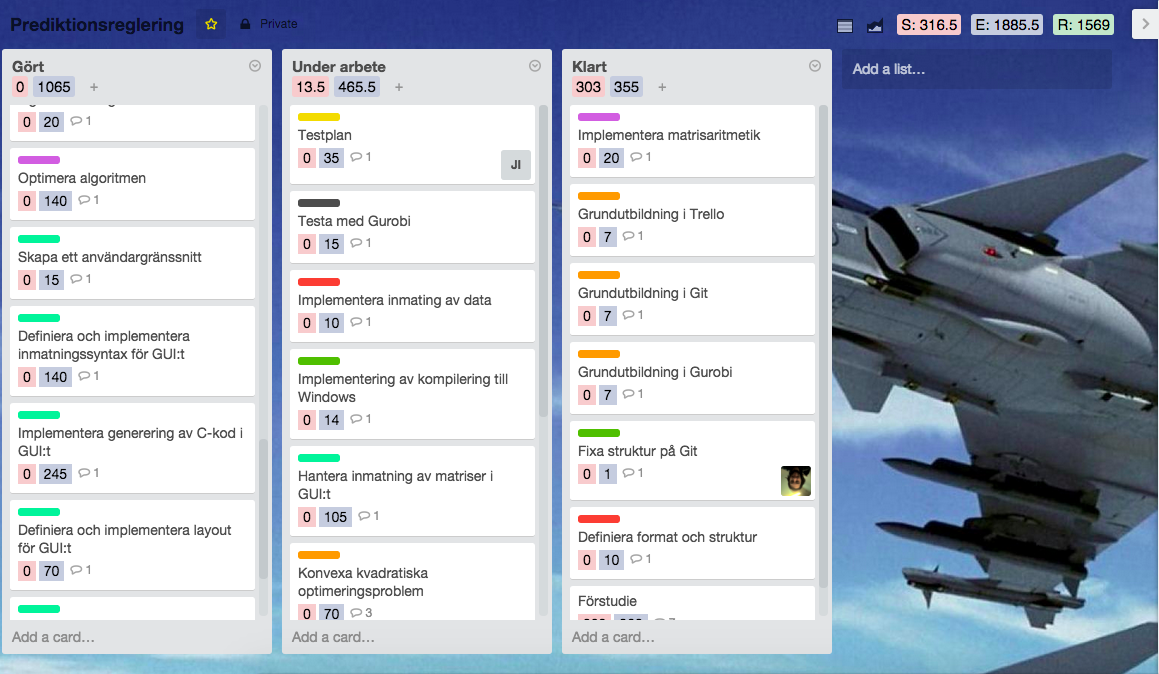
\includegraphics[scale=0.3]{grafik/trello}}
\caption{Scrum table i Trello}
\label{fig:trello}
\end{figure}

\noindent Efter dessa försök med ''Trac'' och ''Trello'' gav kandidatgruppen upp med tanken av att använda utvecklingsmetodiken ''Scrum'' och inledde första iterationen av projektet utan någon specifik utvecklingsmetodik.

\subsubsection{Resterande iterationer}
Som nämnt gick kandidatgruppen in i första iterationen utan någon specifik utvecklingsmetodik, men under arbetetsgången växte en sorts utvecklingsmetodik fram.
\newline
\newline
Under projektet arbetade samtliga gruppmedelmmar i närheten av varandra. I ett tidigt skede hade gruppen tillgång till ett kontor där arbetet kunde genomföras samt möten kunde hållas. Genom att arbeta så nära varandra underlättade det att hjälpa till där det behövdes och om ett problem uppstod kunde det snabbt tas itus med.
\newline
\newline
Den utvecklingsmetodik som växte fram för kandidatgruppen kan efterlikna utvecklingsmetodiken ''eXtreme programming'' också kallad XP. XP är likt ''Scrum'', ett agilt arbetssätt för mjukvaruprojekt. XP innehåller ett antal ''practices'', dvs metoder för hur man ska behandla kod. De metoder som förekommer i kandidatgruppen, finns listade nedan.
\begin{itemize}
  \item \textbf{Pairprogramming} - I kandidatgruppen har vissa medlemmar parprogrammerat. Detta innebär att två stycken personer ska utföra en uppgift, en skriver kod och den andra granskar. Ett byte av roller sker också emellanåt. Genom att parprogrammera kan man diskutera om vad som skulle ge upphov till den bästa lösningen.
  \item \textbf{Refactoring} - ''Refactoring'' är något som har dykt upp väldigt mycket under arbetsgången. Poängen med ''Refactoring'' är att förbättra kods läsbarhets samt reducera komplexiteten utan att ändra kodens syfte. Detta har varit en stor del av projektet då kunden har tryckt på att kod ska vara väldokumenterad och strukturerad.
  \item \textbf{Continuous integeration} - ''Continuous integration'' eller CI som det brukar kallas har också varit en stor del av kandidatprojektet. Det är väldigt viktigt att all kod som skrivs funkar med de olika komponenterna i detta projekt, t.ex. att matrisbiblioteket och koden för lösaren funkar tillsammans. Det som har gjorts i projektet är att tester skrivs för de allra viktigaste funktioner och dessa testas kontinuerligt genom att använda ''Travis CI''. ''Travis CI'' kompilerar all kod och säger till om testerna misslyckas eller inte. CI står för kontinuerlig integration.
\end{itemize}
Med hjälp av dessa ''practices'' och god kommunikation mellan gruppmedlemmarna kunde projektet genomföras. 

\subsection{Forskningsmetod}

